According to QCD, the colour factor of gluons is larger than that of quarks by factor 9/4 ("Casimir ratio")~\cite{ALTARELLI1977298}, which makes gluons emit more particles in the hadronisation than quarks. As a result, a gluon-initiated jet has more charged multiplicity associated and its width is larger than that of a quark-initiated jet. Therefore, the information of the track multiplicity inside a jet is crucial to distinguish quarks from gluons.

The $q/g$ tagging variables used in this study are based on the track multiplicity and are specified as : number of tracks ($\ntrk$), jet width (\wtrk)~\cite{Aad_2014,PhysRevLett.110.212001}, and two point energy correlation function (\cbeta)~\cite{Moult:2016cvt,Larkoski:2013eya} computed from the associated tracks. The expressions are defined as follows:

\begin{description}

  \item[\ntrk] \mbox{} \\
    \ntrk~is a number of tracks associated with the jet. %
    \begin{equation}
    \ntrk = \sum_{\mrm{trk}\in\mrm{jet}}
    \end{equation}

  \item[\wtrk] \mbox{} \\
    \wtrk~is a track-\pt-weighted width of the jet divided by the scalar sum of track transverse momenta. %
    It is defined as %
    \begin{equation}
      \wtrk = \frac{ \sum_{\mrm{trk}\in\mrm{jet}}\pttrk\Delta R_{\mrm{trk,jet}} }{ \sum_{\mrm{trk}\in\mrm{jet}}\pttrk },
    \end{equation}
    where \pttrk~is a \pt~of a charged track reconstructed by the ID and %
    $\Delta R_{\mrm{trk,jet}}$ is a distance in the $\eta-\phi$ plane between the track and the jet axis. %

  \item[\cbeta] \mbox{} \\
    Two point energy correlation function is defined as %
    \begin{equation}
      \cbeta = \frac{ \sum_{i, j\in\mrm{jet}}^{i\neq j} p_{\mrm{T}, i}p_{\mrm{T}, j} \left( \Delta R_{i,j} \right)^{\beta=0.2} }%
        { \left( \sum_{\mrm{trk}\in\mrm{jet}} \pttrk  \right)^{2} }, 
    \end{equation}
    where $i$ and $j$ denote tracks associated with the jet and the sum runs over all the combination of two tracks. % 
    The $\beta$ is fixed to $0.2$, which is known to be suitable for $q/g$ tagging.%~\cite{ref30}. % 

\end{description}

%\FloatBarrier
\subsubsection{The BDT tagger}

Multivariate Analysis (MVA) is a technique introduced to discriminate signal from background, one type of classification algorithm in MVA is the BDT. A tree structure is built to classify datasets through a sequence of branching binary decisions. Data with desirable features is kept by discriminating algorithm whereas others are rejected. Each decision point made construct a node at each level of the decision tree, and a score is assigned to every classifier that goes into the boosting process based on its error rate. One decision node can have two or more branches to split the datasets. Such procedure is iterated from top to down so that a termination condition such as the minimum number of samples in a node or a maximum depth in a tree depth is met. A diagram of a single decision tree is shown in Figure.~\ref{Fig.bdt}. After all series of cuts are applied, the BDT is defined. Therefore, a cut based on the BDT score can be employed as the most correct classification of datasets.

\begin{figure}[htb] 
	\centering  
	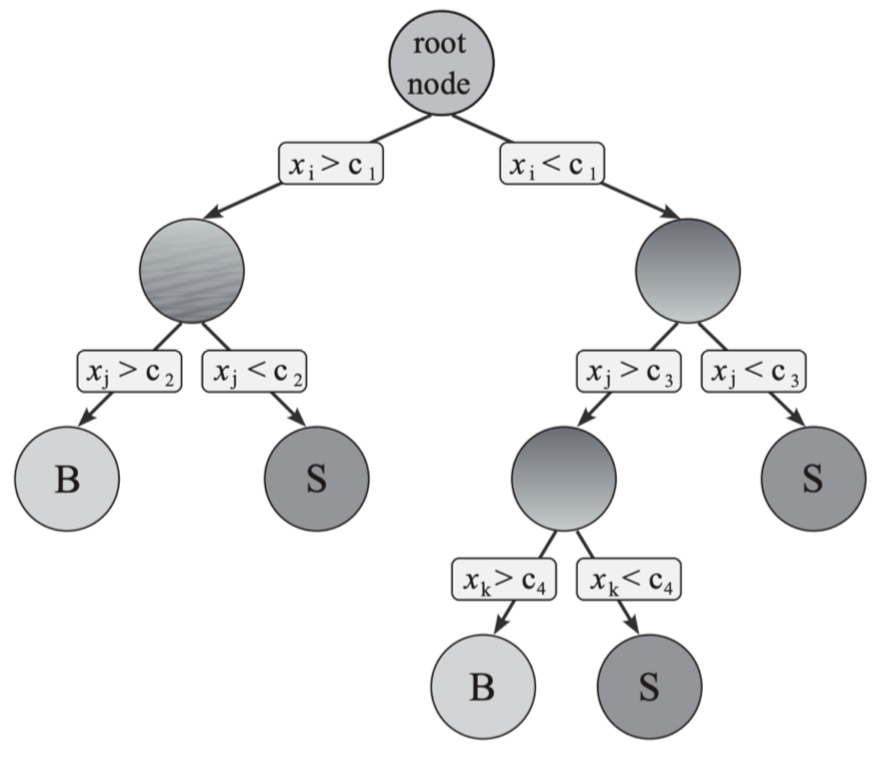
\includegraphics[width=11cm]{./fig/bdt.png}
	\caption{A scheme of a single decision tree with a depth of three}
	\label{Fig.bdt}
\end{figure}

The BDT tagger is constructed by the combination of tracking-related observables: \ntrk, \wtrk, \cbeta~and \pt~of a jet are included as the distribution of the track multiplicity is affected by them. In this study, the BDT score is used to classify quark- or gluon-jets from the multi jet samples, with the truth-labelled information from MC to train until a quark signal efficiency larger than 90\% is reached.


The BDT tagger is trained using the LGBMClassifier from lightGBM~\cite{NIPS2017_6449f44a} framework, and hyper-parameter tuning is performed with Optuna~\cite{akiba2019optuna}. The MC \pythia samples are employed.

An individual score is allocated to each BDT within the boosting procedure, factoring in its error rate.  This BDT score serves as the criterion for classifying a given jet as either a quark-jet or a gluon-jet. 

\paragraph{Feature selections}\mbox{}\par
Drawing upon the features employed during the training process, an exploration of the correlation matrix is undertaken to assess the interdependence among jet attributes, including \pt, \abseta, and jet substructure variables \ntrk, \wtrk, \cbeta, and the BDT. Figure~\ref{fig:weighted_corr} shows \ntrk, \wtrk~and \cbeta exhibit notable interrelationships among themselves, displaying relatively robust correlations. In contrast, \pt~and $\eta$ display a diminished level of correlation. The distributions of all single jet substructure variables and BDT score with systematic uncertainty in forward and central regions are shown in Figure~\ref{fig:QG-pythia-Unc_Ntrk-wp11}. The distributions of all single jet substructure variables and BDT score with systematic uncertainty of quark- and gluon-jets in different \pt~ranges from the MC simulation are shown in Figure~\ref{fig:QG-pythia-Unc_Ntrk-wp11q}.

\begin{figure}[htb]
	\centering
	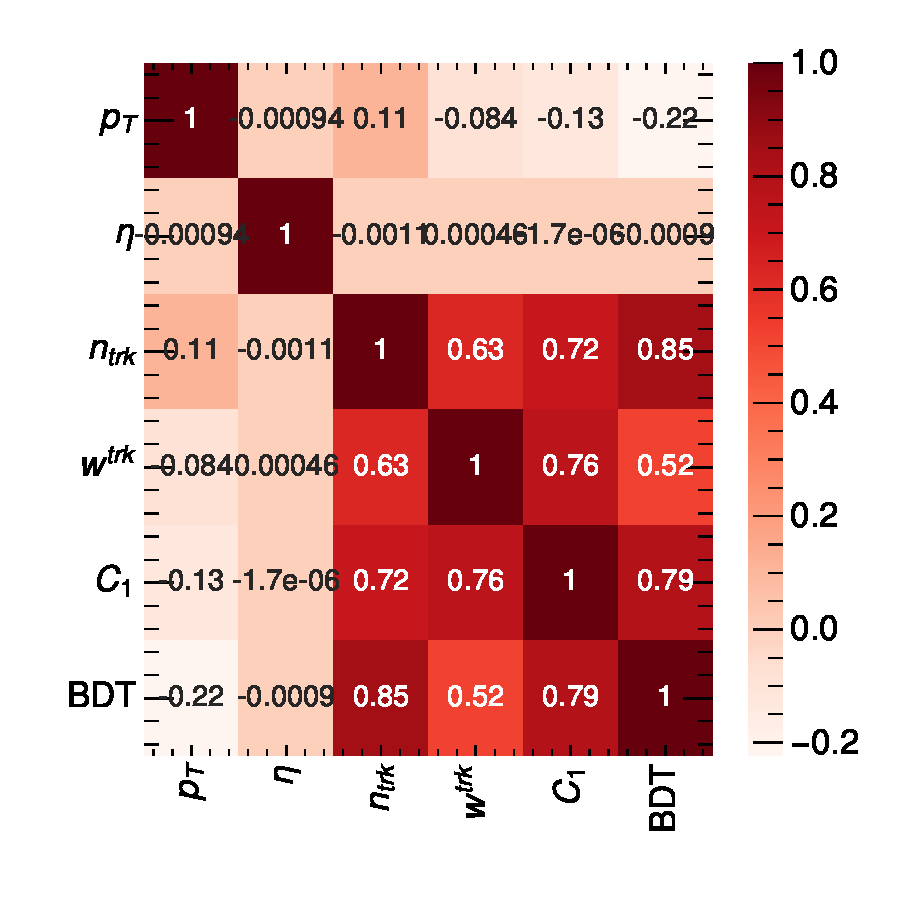
\includegraphics[width=0.65\textwidth]{fig/ADE/new_GBDT/corr.pdf}
	\caption{correlation matrix of jet variables.}
	\label{fig:weighted_corr}
\end{figure}

\begin{figure}[htbp]
	\centering
	\subfloat[]{\label{fig:QG-pythia-UncPythiaQa_Ntrk-wp1}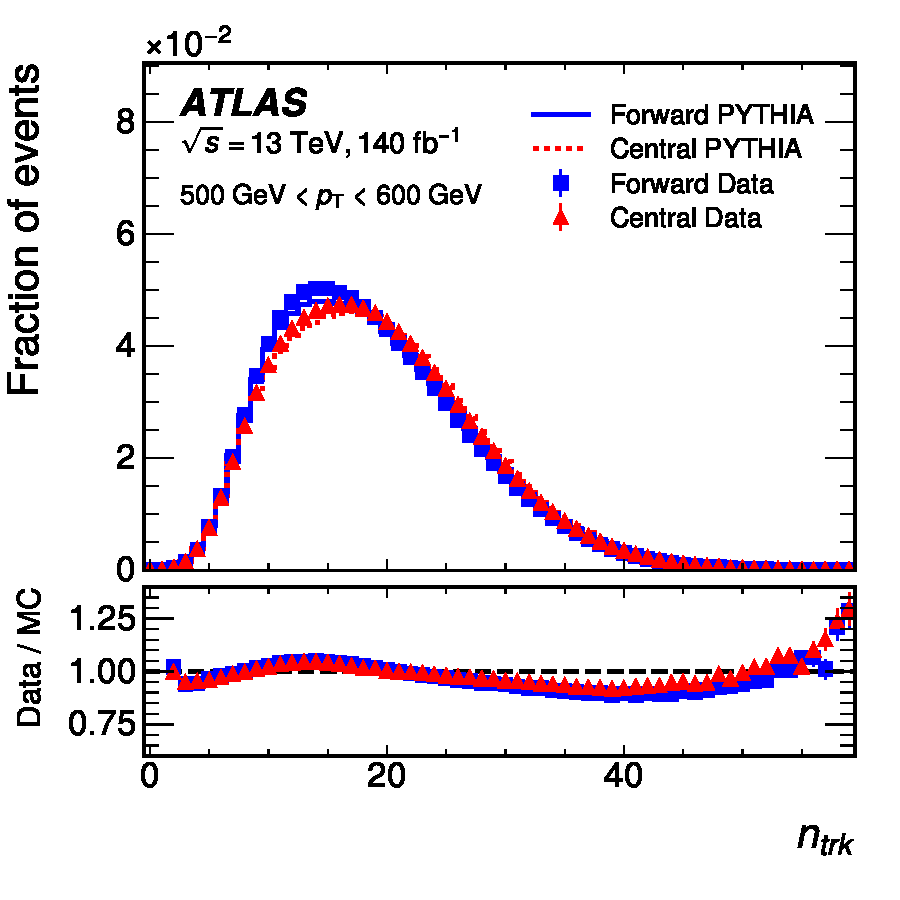
\includegraphics[width=0.45\textwidth]{fig/FvsC_syst/MCvsData_FvsC_500_none_reweight_jet_nTracks.pdf}}\quad
	\subfloat[]{\label{fig:QG-pythia-UncPythiaQb_Ntrk-wp2}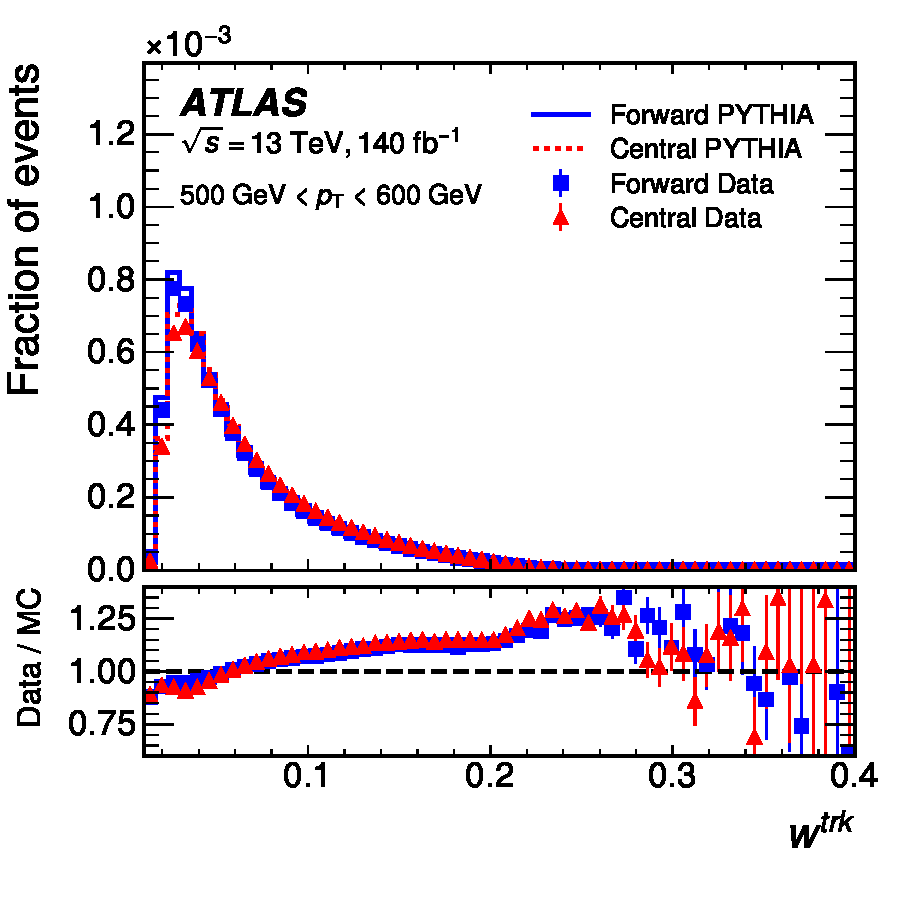
\includegraphics[width=0.45\textwidth]{fig/FvsC_syst/MCvsData_FvsC_500_none_reweight_jet_trackWidth.pdf}}\\
	\subfloat[]{\label{fig:QG-pythia-UncPythiaQa_Ntrk-wp3}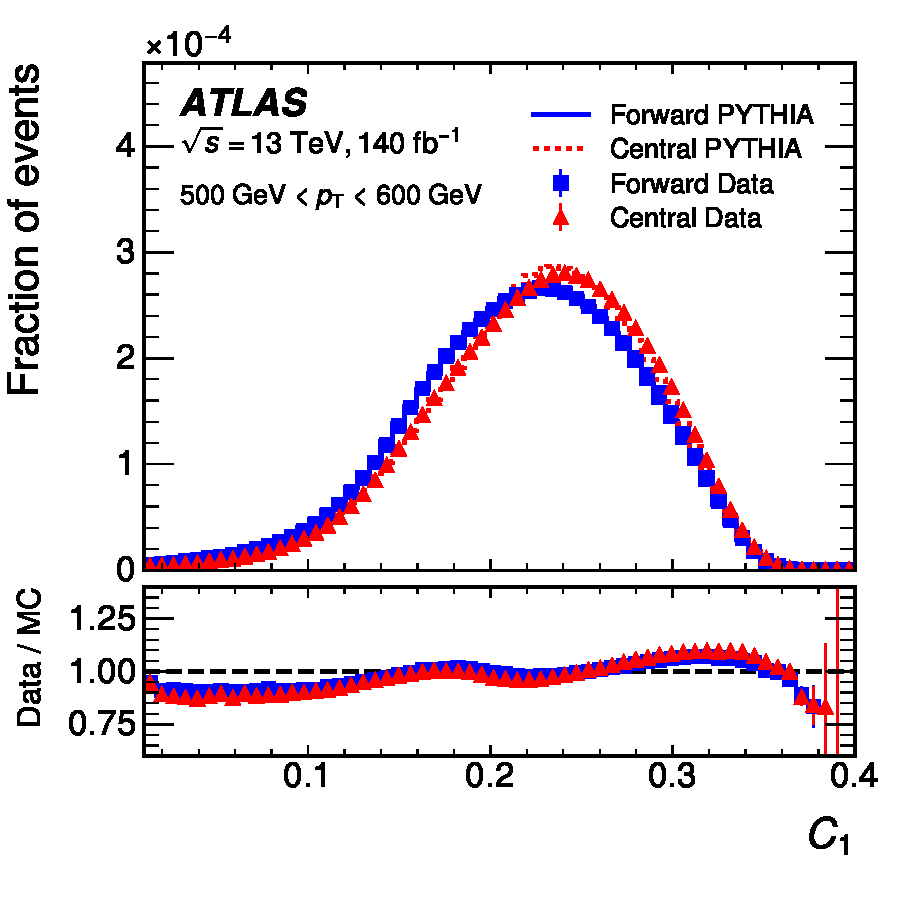
\includegraphics[width=0.45\textwidth]{fig/FvsC_syst/MCvsData_FvsC_500_none_reweight_jet_trackC1.pdf}}\quad
	\subfloat[]{\label{fig:QG-pythia-UncPythiaQb_Ntrk-wp4}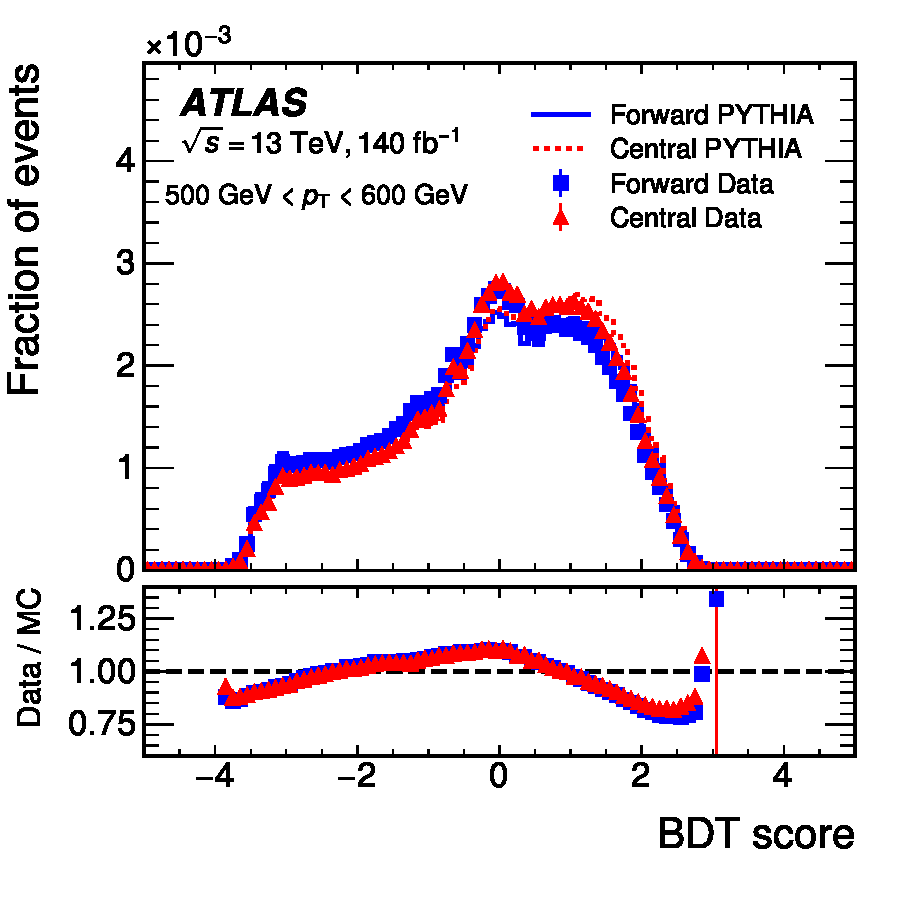
\includegraphics[width=0.45\textwidth]{fig/FvsC_syst/MCvsData_FvsC_500_none_reweight_GBDT_newScore.pdf}}
	\caption[]{
		The distributions of \ntrk~\subref{fig:QG-pythia-UncPythiaQa_Ntrk-wp1}, \wtrk~\subref{fig:QG-pythia-UncPythiaQb_Ntrk-wp2}, $C_1$~\subref{fig:QG-pythia-UncPythiaQa_Ntrk-wp3} and BDT score~\subref{fig:QG-pythia-UncPythiaQb_Ntrk-wp4} in the forward and central regions in data (closed symbols) and the \pythia MC (lines) are shown in the upper panels. The bottom panels show the ratio of the data and the MC. The distributions shown are for jet \pt~in the range between 500 GeV and  600 GeV. The vertical error bars show the statistical uncertainty.
		\label{fig:QG-pythia-Unc_Ntrk-wp11}
	}
\end{figure}


\begin{figure}[htbp]
	\centering
	\subfloat[]{\label{fig:QG-pythia-UncPythiaQa_Ntrk-wp1}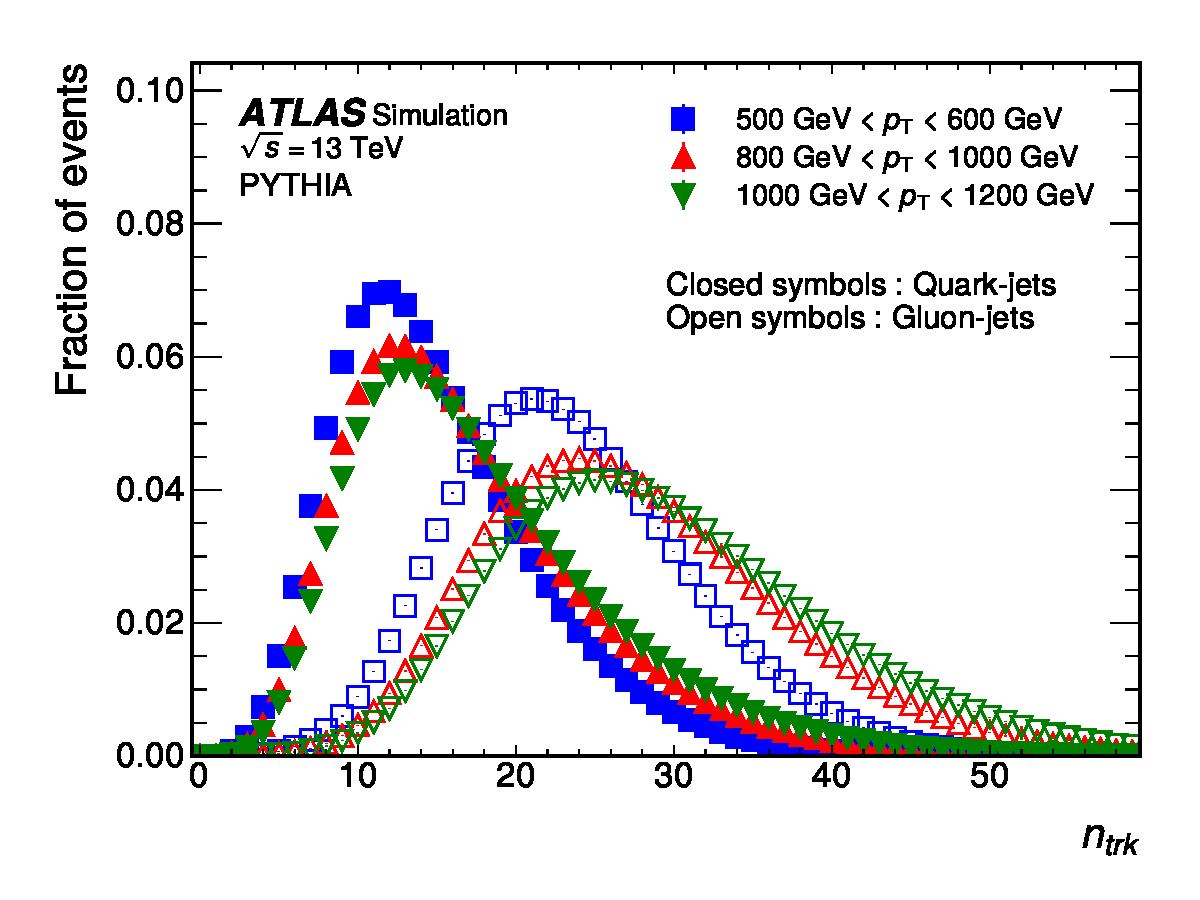
\includegraphics[width=0.45\textwidth]{fig/FvsC_syst/MCvsData_QvsG_1500_none_reweight_jet_nTracks_binned.pdf}}\quad
	\subfloat[]{\label{fig:QG-pythia-UncPythiaQb_Ntrk-wp2}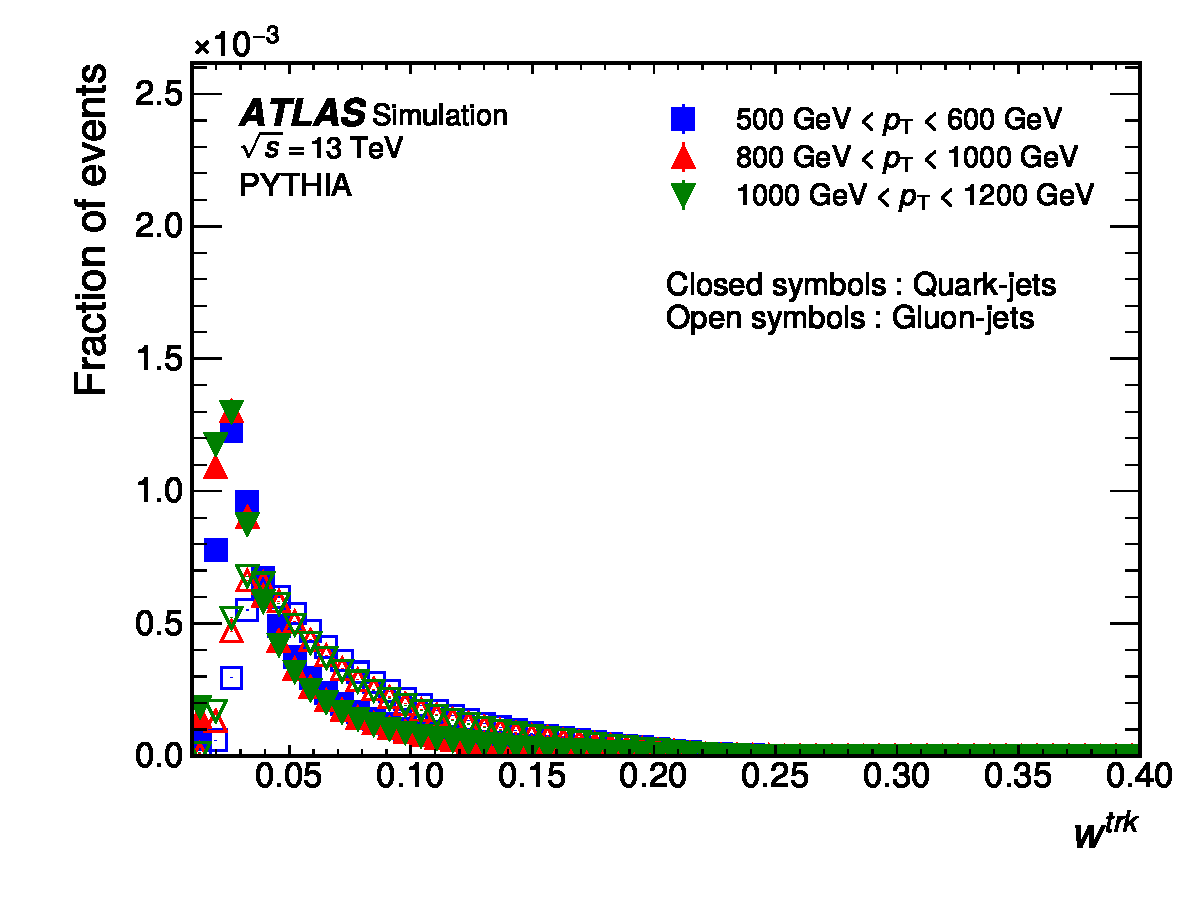
\includegraphics[width=0.45\textwidth]{fig/FvsC_syst/MCvsData_QvsG_1500_none_reweight_jet_trackWidth_binned.pdf}}\\
	\subfloat[]{\label{fig:QG-pythia-UncPythiaQa_Ntrk-wp3}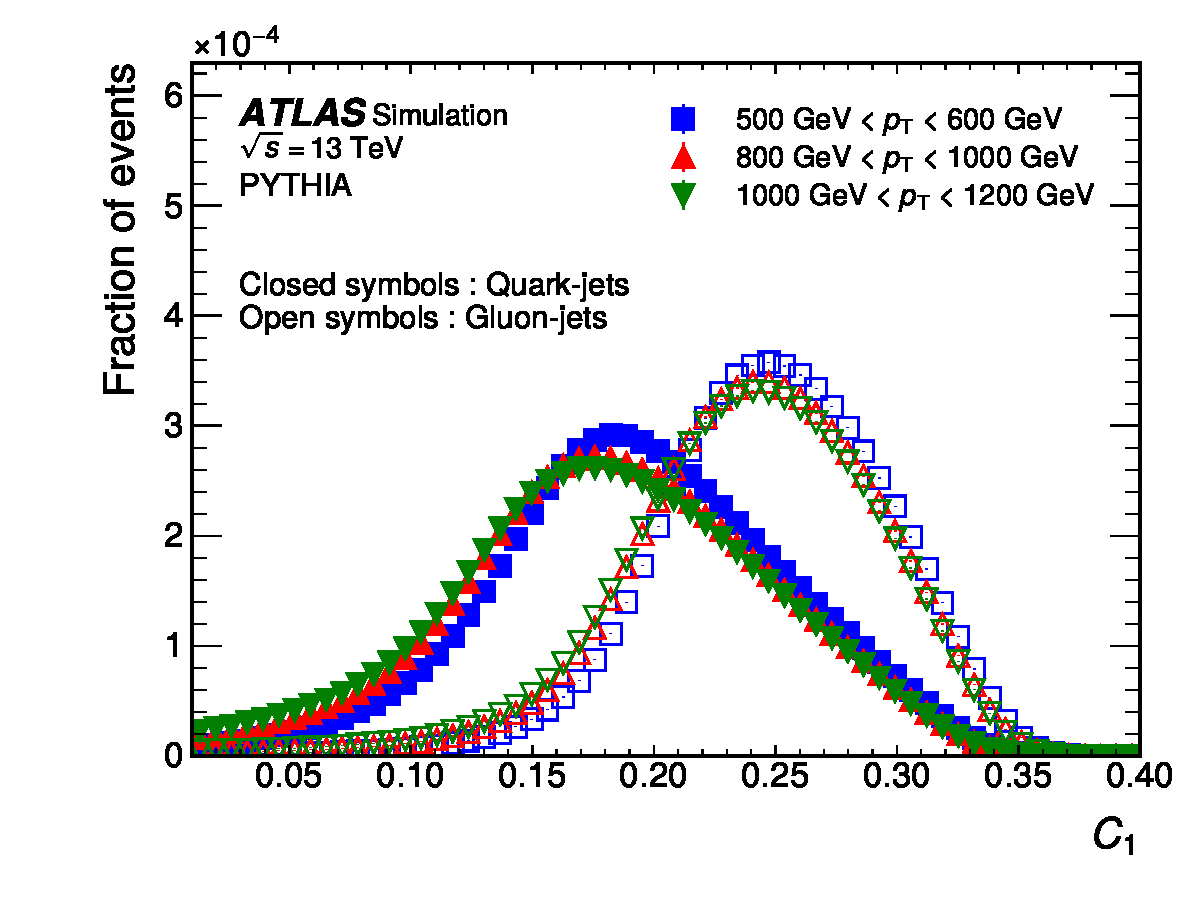
\includegraphics[width=0.45\textwidth]{fig/FvsC_syst/MCvsData_QvsG_1500_none_reweight_jet_trackC1_binned.pdf}}\quad
	\subfloat[]{\label{fig:QG-pythia-UncPythiaQb_Ntrk-wp4}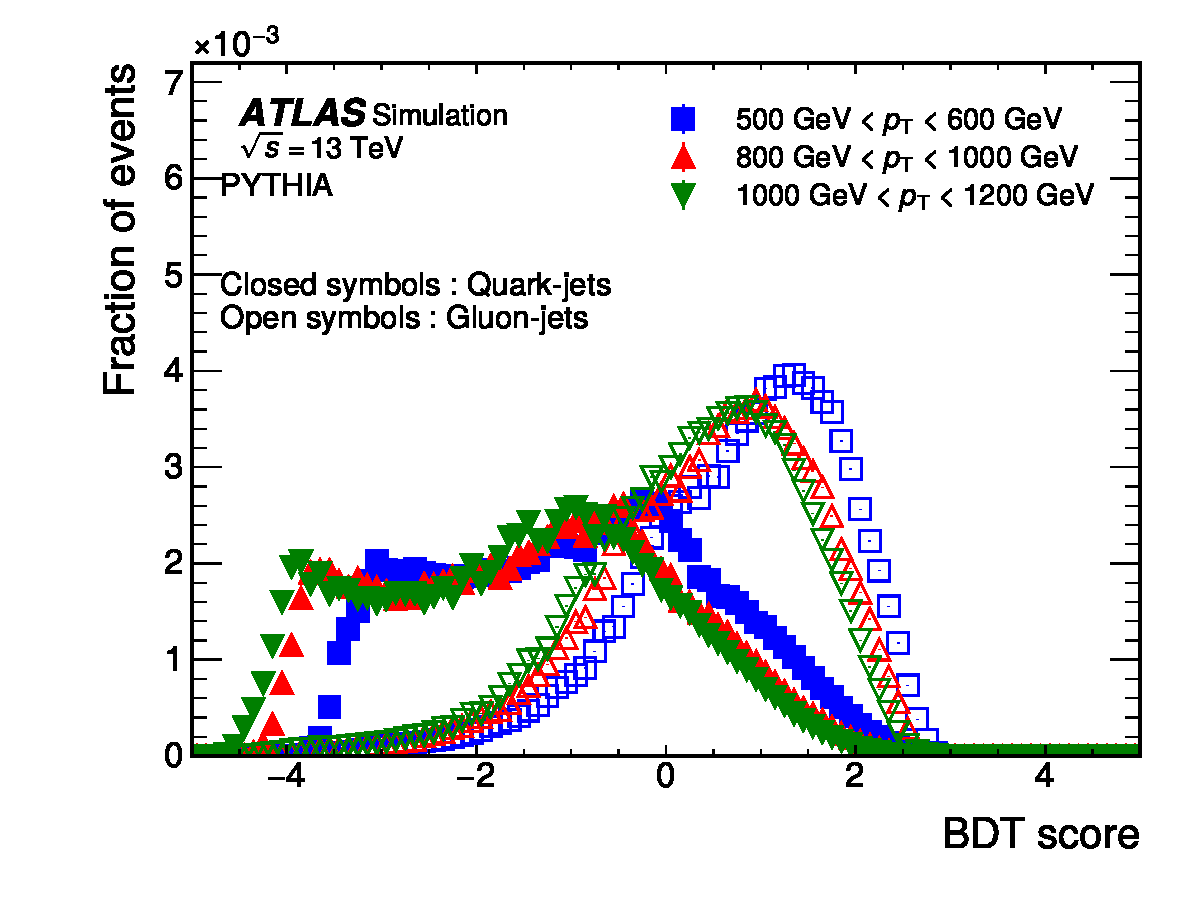
\includegraphics[width=0.45\textwidth]{fig/FvsC_syst/MCvsData_QvsG_1500_none_reweight_GBDT_newScore_binned.pdf}}
	\caption[]{
		The distributions of \ntrk~\subref{fig:QG-pythia-UncPythiaQa_Ntrk-wp1}, \wtrk~\subref{fig:QG-pythia-UncPythiaQb_Ntrk-wp2}, $C_1$~\subref{fig:QG-pythia-UncPythiaQa_Ntrk-wp3} and BDT score~\subref{fig:QG-pythia-UncPythiaQb_Ntrk-wp4} in the quark-jets (closed symbols) and gluon-jets (open symbols) in given \pt~regions using the \pythia MC samples.
		\label{fig:QG-pythia-Unc_Ntrk-wp11q}
	}
\end{figure}

Rather than employing multiple BDTs for different \pt~ranges, an universal BDT can be trained using events in all \pt~ranges.
Given the intrinsic correlation between \ntrk~and the jet \pt, a natural way to choose features is including \pt~in addition to three $q/g$ tagging variables.    
Concerning the remaining variable, $\eta$, two comparative scenarios are juxtaposed: one involves its inclusion, and the other pertains to its exclusion. This comparison facilitates an assessment of whether or not to incorporate \abseta.

\begin{enumerate}
	\item \pt, \ntrk, \wtrk~and \cbeta
	\item \pt, \abseta, \ntrk, \wtrk~and \cbeta
\end{enumerate}

The result depicted in Figure~\ref{fig:QG-training_scenario_compare_500_600} shows a distinct discrepancy when \abseta is encompassed within the training. 
This violates the assumptions that the partons distribution in more forward and more central regions should not change. Specifically, the distribution of BDT scores for forward quarks substantially diverges from that of central quarks, a trend that is similarly observed for gluons. Moreover, adopting the BDT tagger that incorporates \abseta~would result in inadequate performance for jets situated within the central region when this tagger is applied to a pure sample of quark-jets (e.g., $Z$+jet samples).
In the present analysis, the BDT is endowed with the spectra of \pt, \ntrk, \wtrk, and \cbeta, as exemplified in scenario 1. 
At detector-level, however, the observed radiation pattern within jets no longer remains unaffected by \abseta, owing to variances in the detector material and technology. To counteract this effect, a subsequent re-weighting procedure is implemented, described in Section~\ref{sec:QG-closure}. 

\begin{figure}[htb]
	\centering
	\subfloat[Training without \abseta, scenario 1 ]{\label{fig:QG-training-wo-eta-500}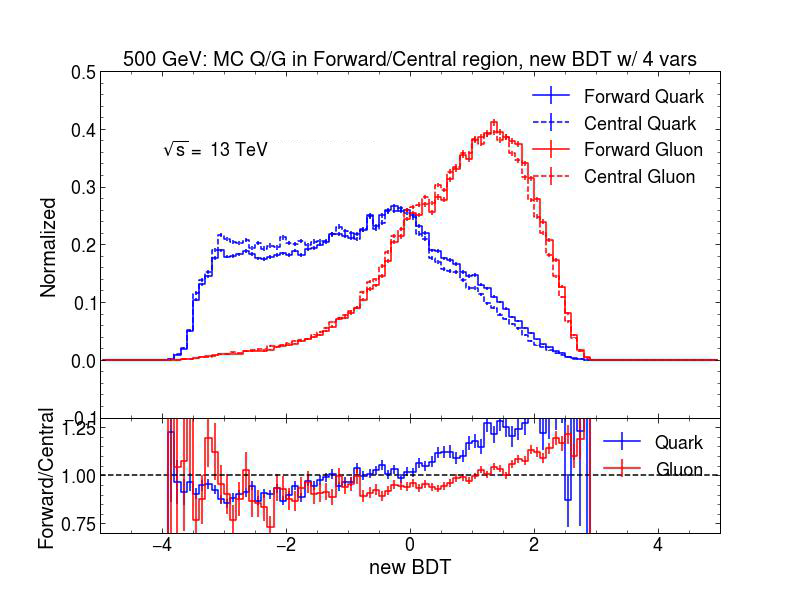
\includegraphics[width=0.45\textwidth]{fig/ADE/new_GBDT/4vars_plots/MC_truth_Q_G_FvsC_500_GBDT_newScore_None.jpg}} \quad
	\subfloat[Training with \abseta, scenario 2]{\label{fig:QG-training-w-eta-500}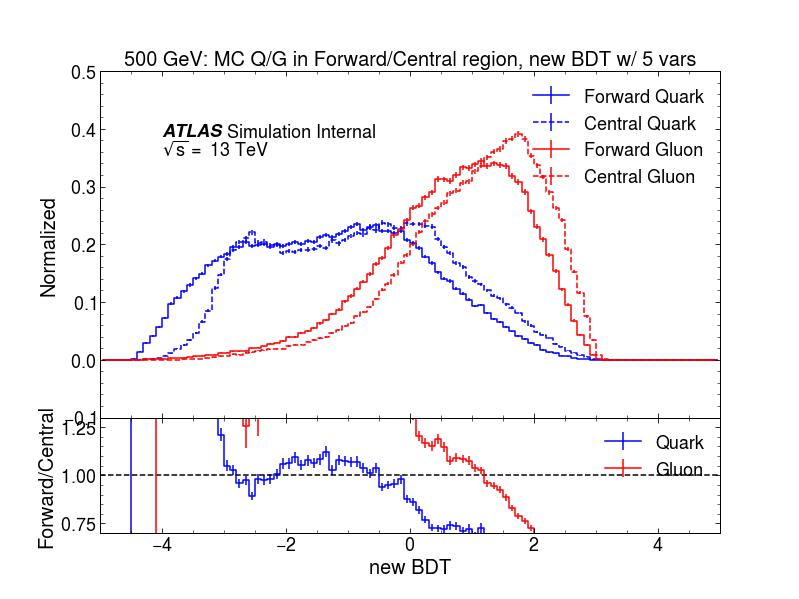
\includegraphics[width=0.45\textwidth]{fig/ADE/new_GBDT/5vars_abseta_plots/MC_truth_Q_G_FvsC_500_GBDT_newScore_None.jpg}}
	\caption[]{
		The comparison of BDT distribution for different scenarios in the jet \pt~range from 500 to 600 GeV. %.
		\label{fig:QG-training_scenario_compare_500_600}
	}
\end{figure}

\paragraph{Training weights}\mbox{}\par
An additional data processing step is conducted to modify the event weights, such that a flat distribution of the \pt~spectrum is given. 
This adjustment is motivated by the observation that higher \pt~jets have less probability to occur, so the training on the higher \pt~jets need to be emphasise. This newly introduced weight, referred to as the "flat \pt-weight" within this context, is exclusively employed during the training process. Conversely, for other scenarios, such as assessing tagger performance on validation datasets and subsequent calibration endeavours, the original event weights based on physical considerations remain employed.

\begin{figure}[htb]
	\centering
	\subfloat[Physical event weight]{\label{fig:QG-training-pt-event-weight}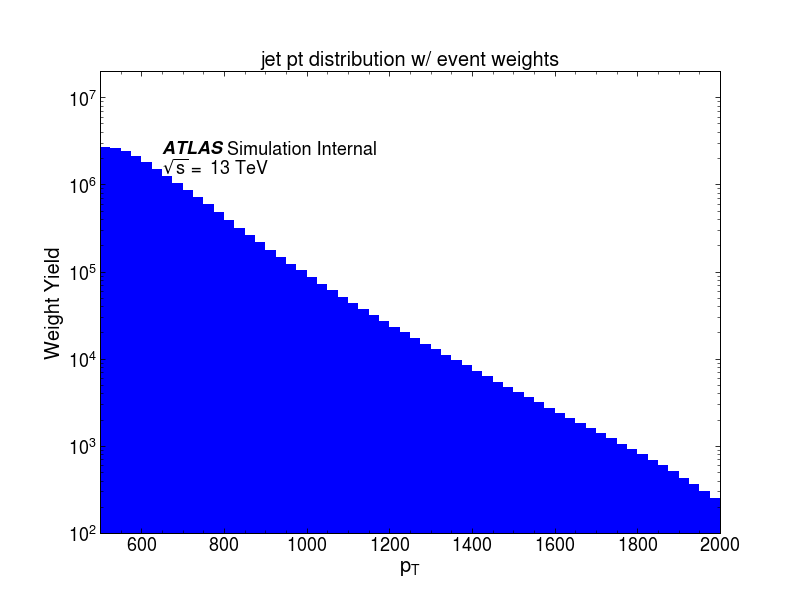
\includegraphics[width=0.45\textwidth]{fig/ADE/new_GBDT/pt_event_weight.png}} \quad
	\subfloat[Flat \pt-weight]{\label{fig:QG-training-pt-flatpt-weight}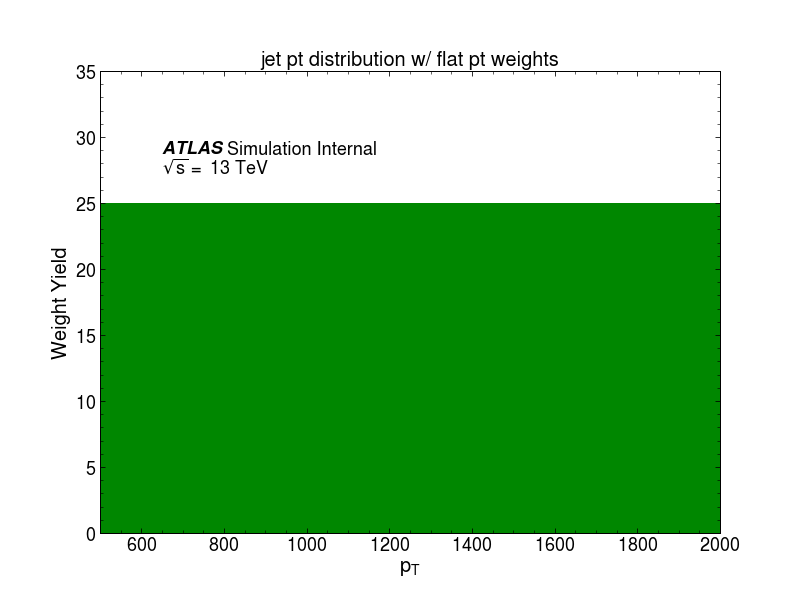
\includegraphics[width=0.45\textwidth]{fig/ADE/new_GBDT/pt_flatpt_weight.png}}
	\caption[]{
		The comparison of jet \pt~distributions with different weights. %.
		\label{fig:QG-training-pt-weight-compare}
	}
\end{figure}

\paragraph{Training Configuration}\mbox{}\par

Approximately 30\% of the data from each period of the MC \pythia8 A, D, E is randomly allocated for the training investigation, constituting an aggregate of roughly 60 million jets. 
The dataset division for training, validation, and testing is structured in a ratio of 80\% for training, 10\% for validation, and 10\% for testing.

Optuna is employed to conduct a search for optimal hyperparameters. Following the hyperparameter tuning process, the most optimal model is achieved after 100 iterations of such procedure. The optimised parameters are listed:

\begin{itemize}
	\item bagging\textunderscore fraction 0.9176347488279626
	\item bagging\textunderscore freq 2
	\item feature\textunderscore fraction 0.9084973008559477
	\item lambda\textunderscore l1 0.0016400096502256838
	\item lambda\textunderscore l0.006327330258011633
	\item min\textunderscore child\textunderscore samples 13
	\item num\textunderscore leaves 224
\end{itemize}

The performance of a classification model at all classification criteria can be illustrated using a receiver operating characteristic (ROC) curve. The idea is to compare the true positive rate (TPR, also known as sensitivity, recall or probability of detection) against the false positive rate (FPR, also known as the probability of false alarm) at different criteria given. Consider a binary classification case, where the outputs are either labelled as positive (p) or negative (n), in total there are four possible outputs from a two-class prediction problem. A true positive (TP) is given if the output from a prediction is p and the actual value is also p, otherwise a false positive (FP) is assigned if the actual value is n. Conversely, a true negative (TN) is given if both the prediction outcome and the actual value are n, whereas a a false negative (FN) is assigned if the actual value is p. TPR as a synonym for recall is defined as:
\begin{equation}
	TPR = TP/(TP+FN)
\end{equation}
while the FPR is defined as: 
\begin{equation}
	FPR = FP/(FP+TN)
\end{equation}

In this analysis, the prediction true is defined by higher \abseta jet and prediction negative is defined by lower \abseta jet. The actual truth value is given by the quark jet from the MC truth information, whereas the actual negative value is given by the gluon truth information. Thus the quark efficiency is the TPR and the gluon rejection is FPR. An Area Under the ROC Curve (AUC) is used to evaluate the performance of a classifier, the better performance is indicated by higher AUC values.

Several ROC plots are made to compare different features and the BDT in different \pt~ranges. 
To check whether the BDT tagger is overtrained, the shape comparison is shown in Figure~\ref{fig:overtraining-validation}, between training dataset and validation dataset.  
No overtraining is observed as the distribution of training dataset is very similar to that of testing dataset. 

Figure~\ref{fig:QG-ROC_500_600} shows the ROC curve for all single jet variables and the BDT-tagger in given \pt~ranges in forward and central regions. Figure~\ref{fig:QG-ROC_800_1000}  shows the AUC of both \ntrk-only tagger and the BDT-tagger as a function of jet \pt. 
\begin{figure}[h]
	\centering
	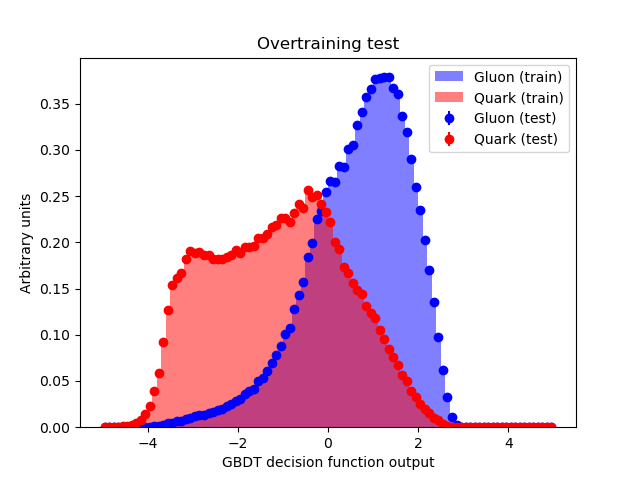
\includegraphics[width=0.65\textwidth]{fig/ADE/new_GBDT/4vars_plots/overtrain_validation.png}
	\caption{Overtraining validation}
	\label{fig:overtraining-validation}
\end{figure}

\begin{figure}[htb]
	\centering
	\subfloat[Forward region ]{\label{fig:QG-NtrkDataMCinclPythiaa}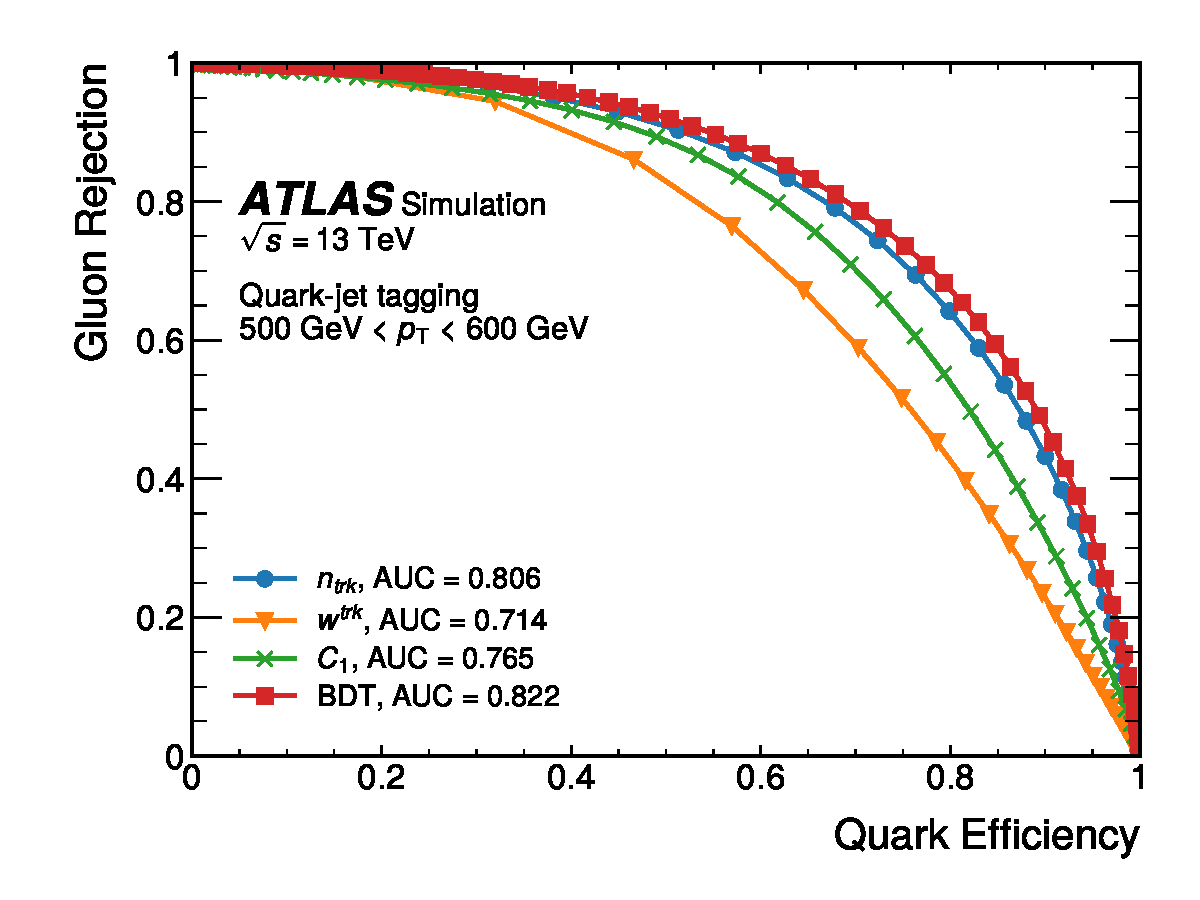
\includegraphics[width=0.48\textwidth]{fig/ROC/ROC_500_Forward_none.pdf}} \quad
	\subfloat[Central region ]{\label{fig:QG-NtrkDataMCinclPythiab}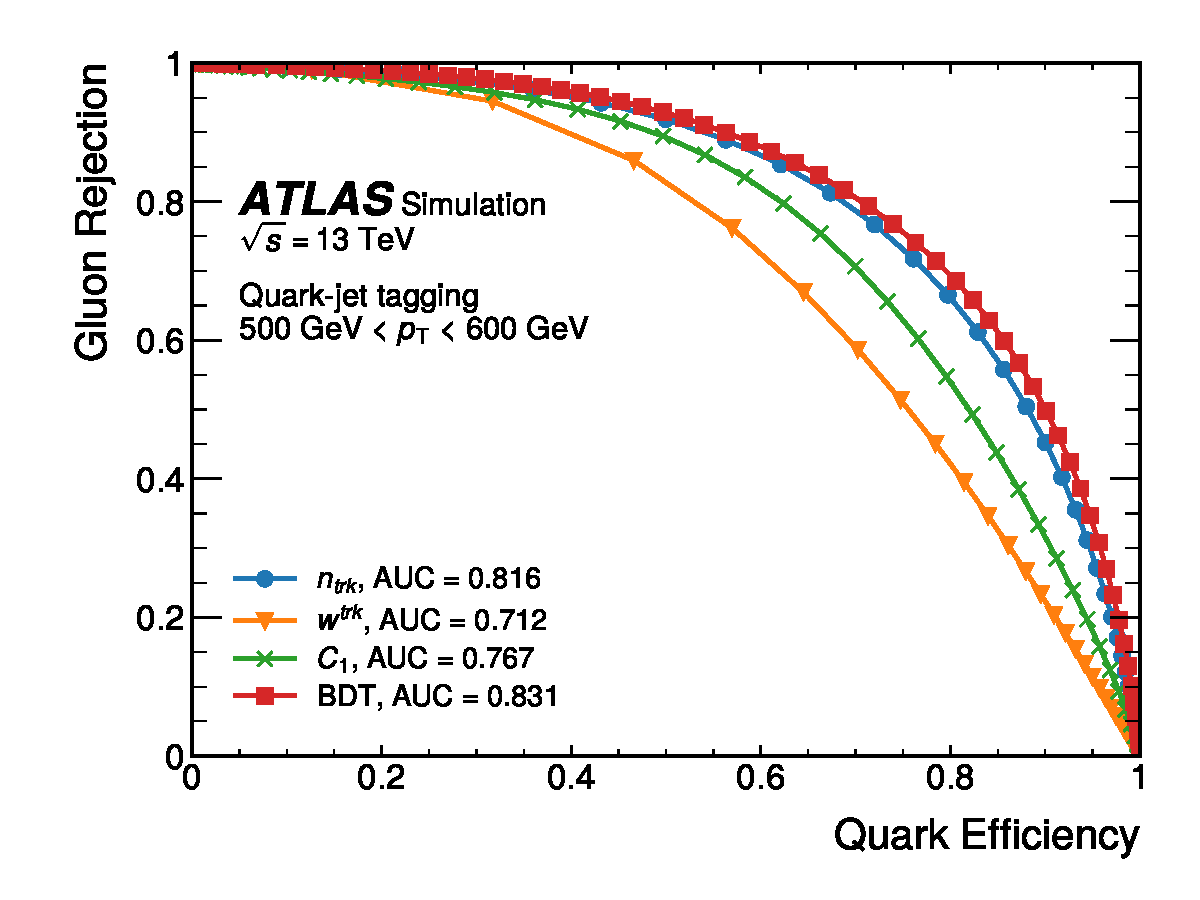
\includegraphics[width=0.48\textwidth]{fig/ROC/ROC_500_Central_none.pdf}}
	\caption[]{
		The ROC Curve for different taggers in the given jet \pt. %.
		\label{fig:QG-ROC_500_600}
	}
\end{figure}


\begin{figure}[htb]
	\centering
	\subfloat[Forward region ]{\label{fig:QG-NtrkDataMCinclPythiaa}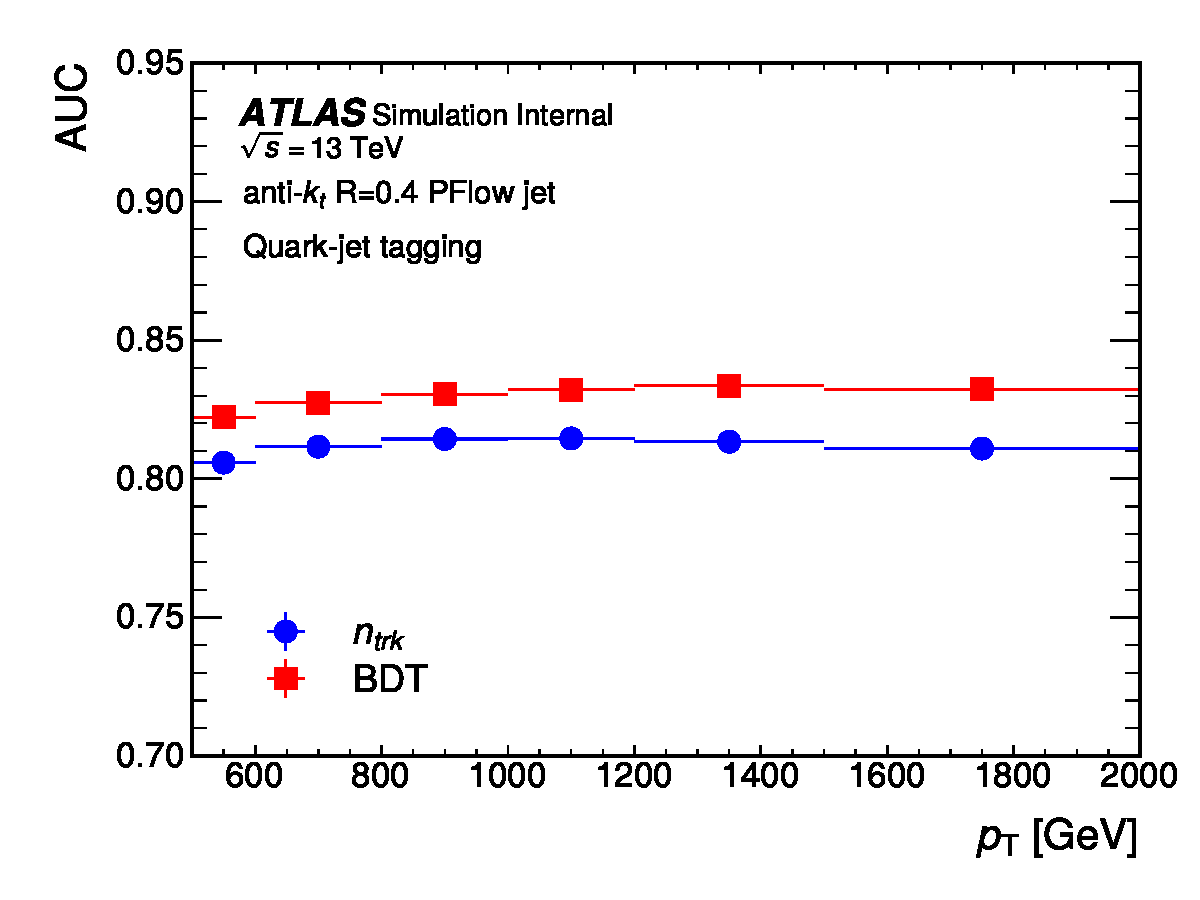
\includegraphics[width=0.48\textwidth]{fig/ROC/pt_Forward_GBDT_newScore.pdf}} \quad
	\subfloat[Central region]{\label{fig:QG-NtrkDataMCinclPythiab}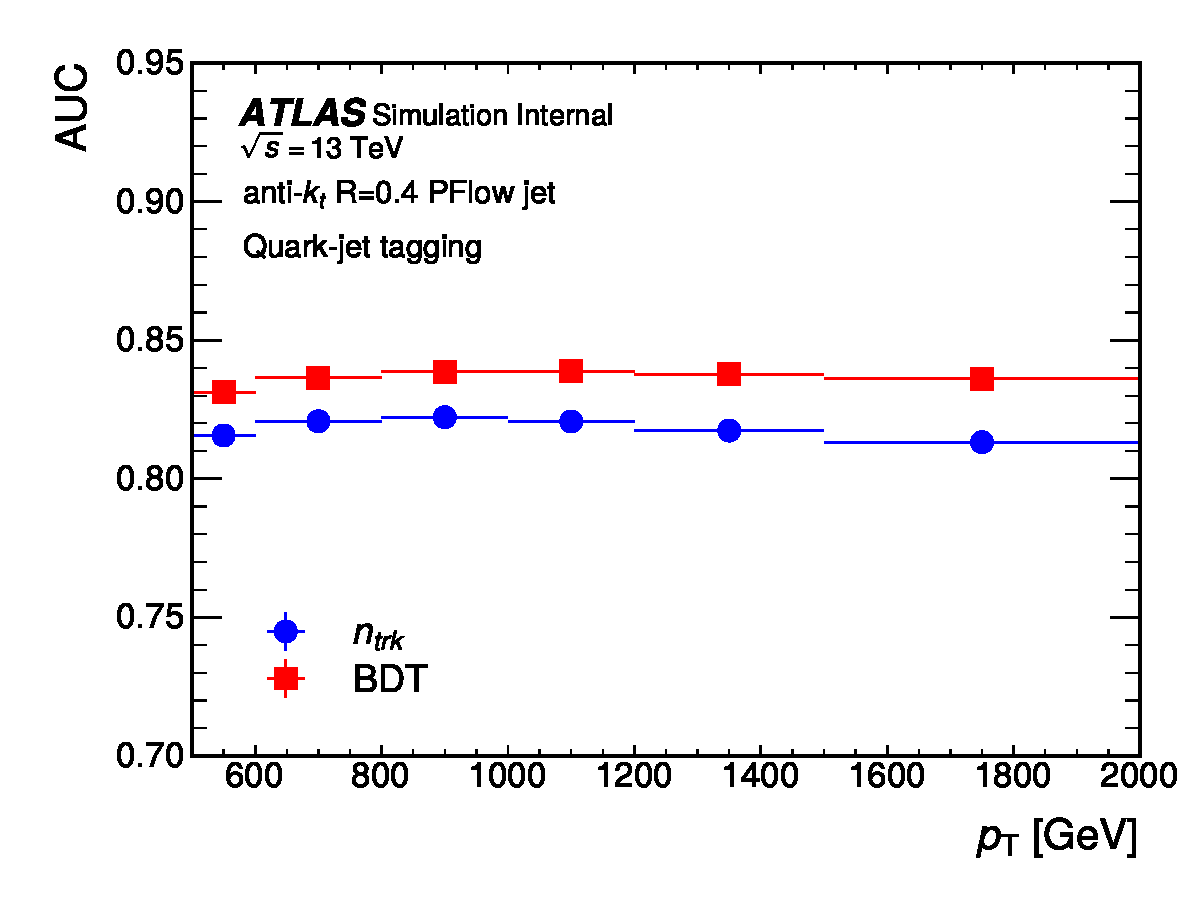
\includegraphics[width=0.48\textwidth]{fig/ROC/pt_Central_GBDT_newScore.pdf}}
	\caption[]{
		The AUC for different taggers across jet \pt. %.
		\label{fig:QG-ROC_800_1000}
	}
\end{figure}

%A receiver operating characteristic (ROC) curve,  is a graph showing the performance of a classification model at all classification thresholds. The ROC curve is created by plotting the true positive rate (TPR) against the false positive rate (FPR) at various threshold settings. The true-positive rate is also known as sensitivity, recall or probability of detection. The false-positive rate is also known as the probability of false alarm and can be calculated as (1-specificity).
%
%Consider a two-class prediction problem (binary classification), in which the outcomes are labeled either as positive (p) or negative (n). There are four possible outcomes from a binary classifier. If the outcome from a prediction is p and the actual value is also p, then it is called a true positive (TP); however, if the actual value is n then it is said to be a false positive (FP). Conversely, a true negative (TN) has occurred when both the prediction outcome and the actual value are n, and a false negative (FN) is when the prediction outcome is n while the actual value is p.
%
%TPR is a synonym for recall and is therefore defined as follows: TPR $=$ TP/(TP+FN), while the FPR is defined as follows: FPR $=$ FP/(FP+TN). In this analysis,  \abseta jet is defined as the prediction true and central \abseta jet is defined as the prediction negative, the truth quark-jet from MC simulation is defined as the actual truth value, the gluon-jet is defined as the actual negative value. Thus, the TPR is quark efficiency and FPR is gluon rejection.

%In classification problems, Area Under the ROC Curve(AUC) is used to evluate the classifier performance. The forward AUC values indicate better performance. The AUC are shown in the ROC plots along the legends. 

The \ntrk-only tagger is found to be the most sensitive observable than other individual jet substructure variables for $q/g$ tagging, 
\wtrk~and \cbeta~are less sensitive to the number of tracks inefficiencies because they are defined as ratios, the BDT-tagger which include the $\wtrk$ and $\cbeta$ has better AUC than \ntrk-only tagger across all jet \pt~ranges. This indicates that the BDT-based tagging mechanism has a heightened capacity to discriminate against gluon-jets at the same level of efficiency in identifying quark-jets with \ntrk-only tagger . Both taggers are calibrated in this paper, more details are presented in the next section.

%\wtrk and \cbeta are less sensitive to the number of trackstrack inefficiencies because they are defined as ratios. %only and it has only a small \eta dependency. %
%\texttt{TightPrimary} identified tracks have few fake tracks and only a small \eta dependency. %

%since such a jet substructure information is not used in the conventional SUSY searches and %
%the mis-modeling of the simulation, especially in a gluon, is known in the previous study for q/g tagging in Run1~\cite{QGRun1}. %

\FloatBarrier

